\documentclass{article}
\usepackage{graphicx}

\begin{document}
\section{Question 1}
\setcounter{subsection}{2}
\subsection{}
Time (in seconds) to complete standard training: 1381.1138. \\
Time (in seconds) to complete free adversarial training: 386.9370.
\subsection{}
\begin{center}
\begin{tabular}{||c c c||} 
    \hline
    Model/Task & Accuracy & PGD Success rate \\ [0.5ex] 
    \hline\hline
    Standard & 0.9168 & 0.9025 \\ 
    \hline
    Adv.-trained & 0.8225 & 0.3695 \\
    \hline 
\end{tabular}
\end{center}
Adversarial training significantly decreases the PGD succees rate, i.e increases robustness with the price of a some (around 10\%) decrease in accuracy.
\subsection{}
\begin{center}
\begin{tabular}{||c c c c||} 
    \hline
    m/metric & Time & Accuracy & PGD Success rate \\ [0.5ex] 
    \hline\hline
    4 & 383.8422 & 0.8077 & 0.3808 \\ 
    \hline
    5 & 323.3860 & 0.7900 & 0.3828 \\
    \hline
    6 & 276.1508 & 0.7713 & 0.3963 \\
    \hline
    7 & 258.2459 & 0.7460 & 0.4073 \\
    \hline 
\end{tabular}
\end{center}
It seems that both the benign accuracy, robustness and training time decrease as m increases.
\section{Question 2}
\setcounter{subsection}{1}
\subsection{}
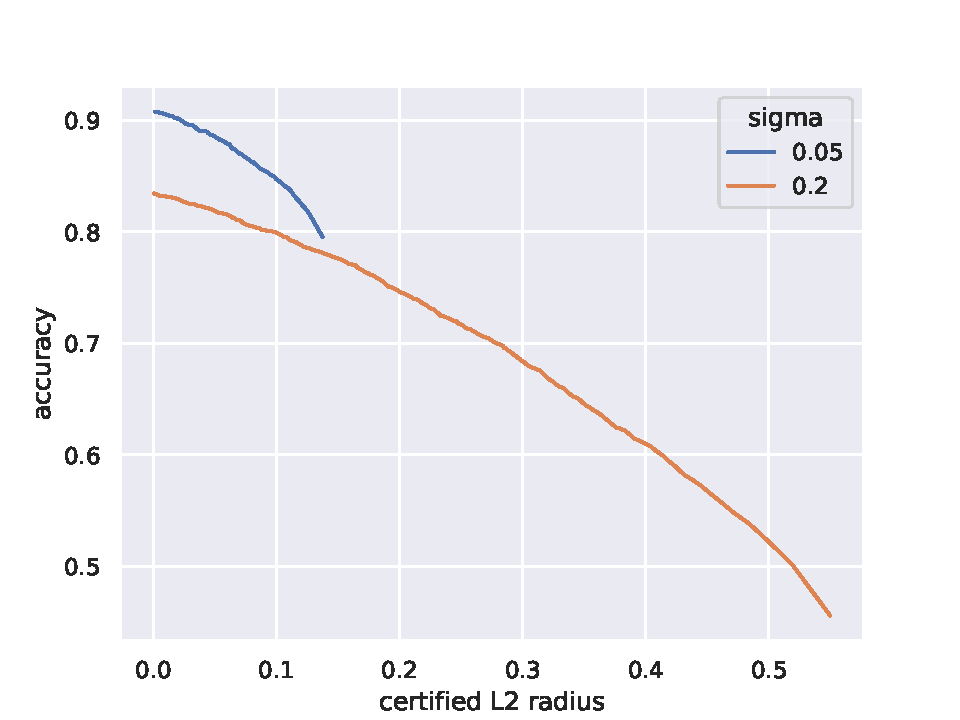
\includegraphics[scale=0.7]{randomized-smoothing-acc-vs-radius.pdf} \\
Let us recall the equation that we've seen in class:
$$R=\sigma \Phi^{-1}(p_c)$$
where $R$ is the radius, $\sigma$ is the standard deviation of the Gaussian noise, 
$\Phi^{-1}$ is the inverse of the CDF of the Gaussian distribution and 
$p_c$ is the confidence level of class $c$. \\
Note that there are two competing factors here: sigma multiplies the value of $R$, hence as $\sigma$ grows larger $R$ grows larger.
On the other hand, as $\sigma$ grows larger, the Gaussian distribution becomes more spread out, this means that the probability of two 
predictions having the same maximum class decreases, hence $p_c$ decreases, which in turn decreases $\Phi^{-1}(p_c)$. \\
It seems that in the range of $\sigma$ that we've tested, the the lower value of $\sigma$, i.e $\sigma=0.05$ has higher accuracy
for a given radius, i.e a larger number of samples with radii bigger then the radius. This means that the second factor we described dominates.
\section{Question 3}
\setcounter{subsection}{1}
\subsection{}
Model 1 is backdoored, the backdoor forces it to output class 0.
\subsection{}
\subsubsection{}
mask: \\

\includegraphics[scale=2]{backdoor-mask.jpg} \\
trigger: \\
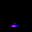
\includegraphics[scale=2]{backdoor-trigger.jpg}
\subsubsection{}
Yes. The accuracy of Model 1 is only very slightly lower than that of Model 2 (0.9107 vs 0.9168).
\subsubsection{}
Very successful, its success rate is 0.9982.
\end{document}

